% !Mode:: "TeX:UTF-8"

\chapter{绪论}

\section{课题研究的背景和意义}

随着计算机和软件技术的不断进步,软件系统的规模和复杂性也随之增长,尤其是那些被称为遗留
系统(legacy system)或遗产软件的项目。这些遗留系统由于其庞大的规模和维护升
级的难度,成为了代码质量分析的重要领域。根据 Chiu 等人的定义[1],遗留系统是指
那些维护和升级难度较高的大规模软件系统。而 Carvalho 等人[2]则将遗留系统描述为
依赖过时技术的系统,这些系统经过多年的广泛维护,导致其架构衰变和退化。遗留系
统的复杂性不仅体现在它们由紧密相连且相互依赖的组件构成,难以扩展和创新[3],还
在于它们对维护资源的巨大需求,这阻碍了数字化转型的步伐。尽管如此,这些系统代
表着长期的大规模投资,包含企业的重要数据和技术流程,完全抛弃可能会导致重要资
产流失,不可轻易放弃。因此,为了保持竞争力和保护现有投资,许多公司都选择对这
些遗留系统进行继续维护或者重构。

除了遗留系统之外,对于一般的软件项目,持续维护也是最重要的代码活动之一。调查显示,软件系统的维护成本在历年的软件维护预算中占 60\%到 80\%的比重[4]。标准的代码维护工作的流程图如图1-1所示,主要分为以下三个步骤:

(1)开发人员进行代码开发。修改项目代码后,针对修改部分进行回归测试,验证功能是否符合需求,同时避免缺陷的引入。

(2)测试通过后,由审查人员进行代码审查。代码审查的主要目的是确保代码质量,通过识别潜在的错误和优化点,提升代码的可维护性与可靠性,同时保证开发风格的统一。

(3)审查通过后,则可与原始项目进行合并。

\begin{figure}[h]
\centering
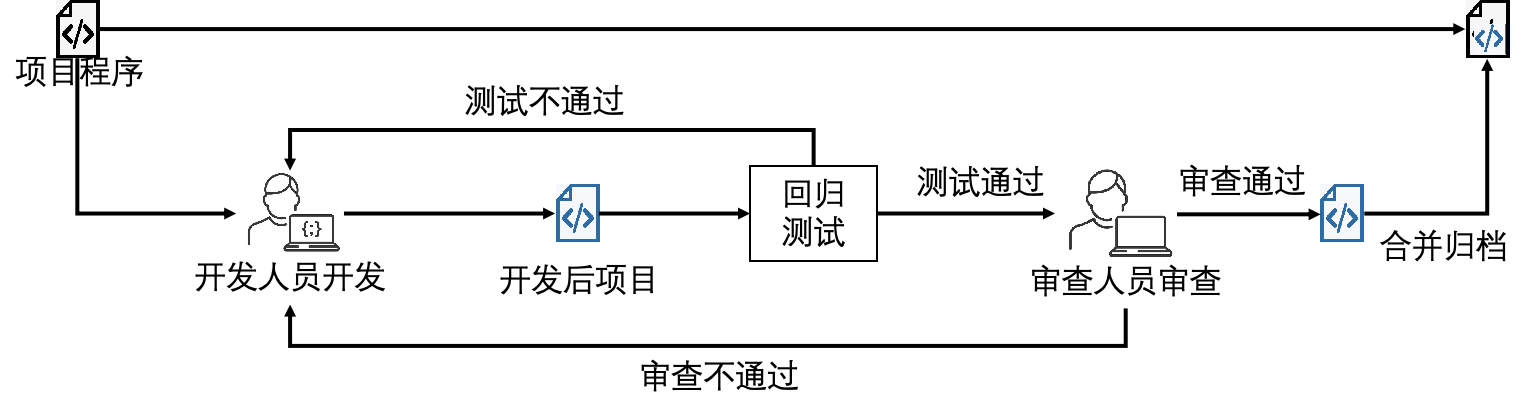
\includegraphics[width = 0.9\textwidth]{开发审查流程.png}
\caption{示例代码}
\end{figure}

软件项目由于历史原因,往往存在大量低质量代码和技术债务。在对软件项目进行维护或重构的过程中,代码质量分析是具有指导性意义的关键一环。代码质量分析可以帮助开发者识
别代码质量问题和问题所在的位置,提供有针对性的优化以及重构方案,从而降低成本和风险。通过有效的代码质量分析,企业可以逐步提升软件系统的稳定性和可维护性,为实现数字化转型打下坚实基础。这不仅能够保护企业的长期投资,还能提升整体竞争力,确保在快速变
化的市场中保持领先地位。

代码变更影响分析是代码质量分析的重要方法之一。通过代码变更影响分析,能够确定当某处代码进行变更时,系统中的其他哪些部分会受到影响,这可以让开发人员提前了解与变更部分有依赖关系的其他模块,避免变更时引入问题。

对于大型软件系统,代码变更影响分析更显得尤为关键。大型软件系统往往融合了不同开发者的个性化风格,随着时间的推移,系统的模块化设计原则逐渐被繁复和庞大的代码结构所淹没。这种情况下,精准地识别变更后有影响的代码模块,对于系统的有效重构和维护至关重要。然而,传统依赖经验丰富的专家
进行手工提取的方法,在面对日益复杂化的系统结构时,显得力不从心[5]。因此,从代
码变更影响分析的角度出发,不仅能深入理解代码变更对系统整体和各个子模块的潜在
影响,还能够提高维护项目的效率[6]。这种方法为软件系统的维护和升级提供了一种更
为科学和系统的解决策略,有助于实现软件质量的持续提升和维护成本的有效控制。

本文将从代码变更影响分析入手进行方法研究,面向代码质量评估,同时结合静态分析方法对代码项目进行代码度量提取和缺陷检测,帮助开发者和审查人员更直观地理解整个项目,为维护项目代码提供更有效的保障。

\section{国内外研究现状及分析}


\subsection{代码质量分析的国内外研究现状}

软件质量与软件的稳定性、可靠性、健壮性、可维护性等关键特性密切相关,是衡量软件性能和可靠性等指标的重要标准。作为软件质量的重要组成部分,代码质量在整体软件质量中占据着至关重要的地位,直接影响着软件系统的长期可用性与可维护性。

在分析代码质量时,按照主题主要可以分为以下几种,

(1)代码缺陷

(2)代码复杂度

(3)代码变更

(4)代码内聚度

(5)代码耦合性

除此之外,还包括代码可重用性、代码可读性、代码性能、代码安全性等研究主题。

根据不同的研究主题,演化出了很多代码度量套件,用于评估代码质量的高低。


\subsection{代码变更影响分析方法}


\section{本文的主要研究内容以及各章节安排}
\subsection{主要研究内容}
\subsection{章节安排}


